\documentclass{standalone}
\usepackage{tikz}
\usetikzlibrary{patterns, positioning}

\begin{document}
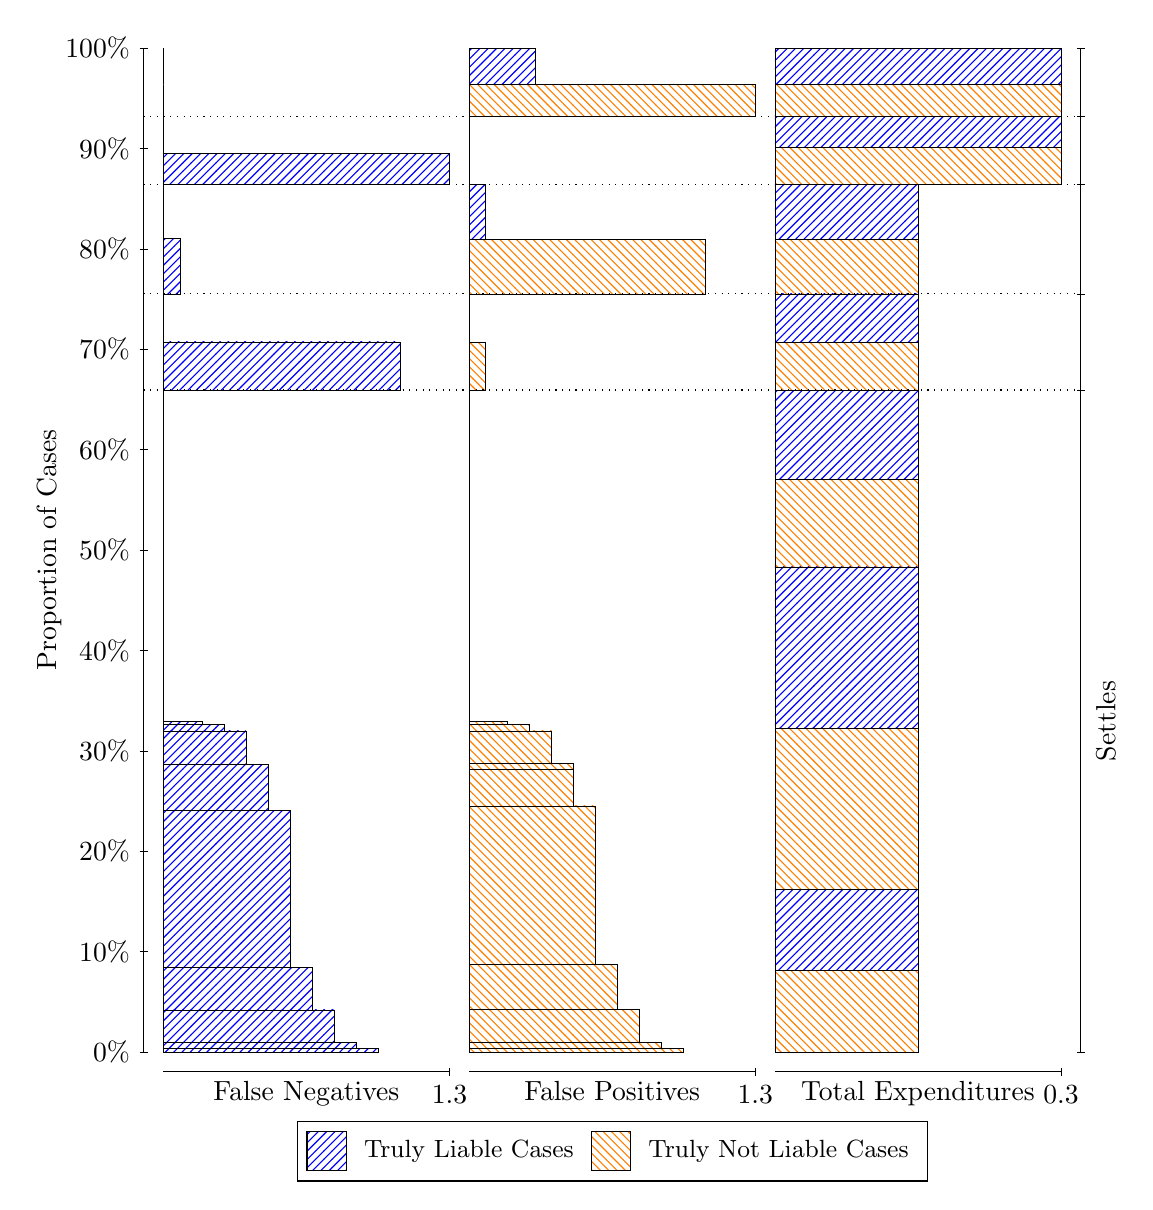
\begin{tikzpicture}
\draw[black, very thin] (1.5,1.75) -- (1.5,14.5);
\node[rotate=90, anchor=center] at (0.3, 8.125) {Proportion of Cases};
\draw[black, very thin] (1.45,1.75) -- (1.55,1.75);
\node[anchor=east] at (1.45, 1.75) {0\%};
\draw[black, very thin] (1.45,3.025) -- (1.55,3.025);
\node[anchor=east] at (1.45, 3.025) {10\%};
\draw[black, very thin] (1.45,4.3) -- (1.55,4.3);
\node[anchor=east] at (1.45, 4.3) {20\%};
\draw[black, very thin] (1.45,5.575) -- (1.55,5.575);
\node[anchor=east] at (1.45, 5.575) {30\%};
\draw[black, very thin] (1.45,6.85) -- (1.55,6.85);
\node[anchor=east] at (1.45, 6.85) {40\%};
\draw[black, very thin] (1.45,8.125) -- (1.55,8.125);
\node[anchor=east] at (1.45, 8.125) {50\%};
\draw[black, very thin] (1.45,9.4) -- (1.55,9.4);
\node[anchor=east] at (1.45, 9.4) {60\%};
\draw[black, very thin] (1.45,10.675) -- (1.55,10.675);
\node[anchor=east] at (1.45, 10.675) {70\%};
\draw[black, very thin] (1.45,11.95) -- (1.55,11.95);
\node[anchor=east] at (1.45, 11.95) {80\%};
\draw[black, very thin] (1.45,13.225) -- (1.55,13.225);
\node[anchor=east] at (1.45, 13.225) {90\%};
\draw[black, very thin] (1.45,14.5) -- (1.55,14.5);
\node[anchor=east] at (1.45, 14.5) {100\%};

\draw[black, very thin] (13.4,1.75) -- (13.4,14.5);
\draw[black, very thin] (13.35,1.75) -- (13.45,1.75);
\node[anchor=west] at (13.35, 1.75) {};
\draw[black, very thin] (13.35,10.157) -- (13.45,10.157);
\node[anchor=west] at (13.35, 10.157) {};
\draw[black, very thin] (13.35,11.378) -- (13.45,11.378);
\node[anchor=west] at (13.35, 11.378) {};
\draw[black, very thin] (13.35,12.771) -- (13.45,12.771);
\node[anchor=west] at (13.35, 12.771) {};
\draw[black, very thin] (13.35,13.636) -- (13.45,13.636);
\node[anchor=west] at (13.35, 13.636) {};
\draw[black, very thin] (13.35,14.5) -- (13.45,14.5);
\node[anchor=west] at (13.35, 14.5) {};

\draw[black, very thin, pattern color=blue, pattern=north east lines] (1.75,1.75) rectangle (4.475,1.7952);
\draw[black, very thin, pattern color=blue, pattern=north east lines] (1.75,1.7952) rectangle (4.1955,1.8755);
\draw[black, very thin, pattern color=blue, pattern=north east lines] (1.75,1.8755) rectangle (3.916,2.2834);
\draw[black, very thin, pattern color=blue, pattern=north east lines] (1.75,2.2834) rectangle (3.6365,2.823);
\draw[black, very thin, pattern color=blue, pattern=north east lines] (1.75,2.823) rectangle (3.3571,4.8208);
\draw[black, very thin, pattern color=blue, pattern=north east lines] (1.75,4.8208) rectangle (3.0776,5.4003);
\draw[black, very thin, pattern color=blue, pattern=north east lines] (1.75,5.4003) rectangle (2.7981,5.8292);
\draw[black, very thin, pattern color=blue, pattern=north east lines] (1.75,5.8292) rectangle (2.5186,5.9102);
\draw[black, very thin, pattern color=blue, pattern=north east lines] (1.75,5.9102) rectangle (2.2391,5.9532);
\draw[black, very thin, pattern color=orange, pattern=north west lines] (1.75,5.9532) rectangle (1.75,10.157);
\draw[black, very thin, pattern color=blue, pattern=north east lines] (1.75,10.157) rectangle (4.7545,10.769);
\draw[black, very thin, pattern color=orange, pattern=north west lines] (1.75,10.769) rectangle (1.75,11.378);
\draw[black, very thin, pattern color=blue, pattern=north east lines] (1.75,11.378) rectangle (1.9596,12.078);
\draw[black, very thin, pattern color=orange, pattern=north west lines] (1.75,12.078) rectangle (1.75,12.771);
\draw[black, very thin, pattern color=blue, pattern=north east lines] (1.75,12.771) rectangle (5.3833,13.166);
\draw[black, very thin, pattern color=orange, pattern=north west lines] (1.75,13.166) rectangle (1.75,13.636);
\draw[black, very thin, pattern color=orange, pattern=north west lines] (1.75,13.636) rectangle (1.75,14.036);
\draw[black, very thin, pattern color=blue, pattern=north east lines] (1.75,14.036) rectangle (1.75,14.5);
\draw[black, very thin, pattern color=orange, pattern=north west lines] (5.6333,1.75) rectangle (8.3583,1.7917);
\draw[black, very thin, pattern color=orange, pattern=north west lines] (5.6333,1.7917) rectangle (8.0788,1.8706);
\draw[black, very thin, pattern color=orange, pattern=north west lines] (5.6333,1.8706) rectangle (7.7994,2.2915);
\draw[black, very thin, pattern color=orange, pattern=north west lines] (5.6333,2.2915) rectangle (7.5199,2.8642);
\draw[black, very thin, pattern color=orange, pattern=north west lines] (5.6333,2.8642) rectangle (7.2404,4.8754);
\draw[black, very thin, pattern color=orange, pattern=north west lines] (5.6333,4.8754) rectangle (6.9609,5.3437);
\draw[black, very thin, pattern color=orange, pattern=north west lines] (5.6333,5.3437) rectangle (6.9609,5.4176);
\draw[black, very thin, pattern color=orange, pattern=north west lines] (5.6333,5.4176) rectangle (6.6814,5.8277);
\draw[black, very thin, pattern color=orange, pattern=north west lines] (5.6333,5.8277) rectangle (6.4019,5.9082);
\draw[black, very thin, pattern color=orange, pattern=north west lines] (5.6333,5.9082) rectangle (6.1224,5.9533);
\draw[black, very thin, pattern color=blue, pattern=north east lines] (5.6333,5.9533) rectangle (5.6333,10.157);
\draw[black, very thin, pattern color=orange, pattern=north west lines] (5.6333,10.157) rectangle (5.8429,10.765);
\draw[black, very thin, pattern color=blue, pattern=north east lines] (5.6333,10.765) rectangle (5.6333,11.378);
\draw[black, very thin, pattern color=orange, pattern=north west lines] (5.6333,11.378) rectangle (8.6378,12.071);
\draw[black, very thin, pattern color=blue, pattern=north east lines] (5.6333,12.071) rectangle (5.8429,12.771);
\draw[black, very thin, pattern color=orange, pattern=north west lines] (5.6333,12.771) rectangle (5.6333,13.242);
\draw[black, very thin, pattern color=blue, pattern=north east lines] (5.6333,13.242) rectangle (5.6333,13.636);
\draw[black, very thin, pattern color=orange, pattern=north west lines] (5.6333,13.636) rectangle (9.2667,14.036);
\draw[black, very thin, pattern color=blue, pattern=north east lines] (5.6333,14.036) rectangle (6.4718,14.5);
\draw[black, very thin, pattern color=orange, pattern=north west lines] (9.5167,1.75) rectangle (11.333,2.7828);
\draw[black, very thin, pattern color=blue, pattern=north east lines] (9.5167,2.7828) rectangle (11.333,3.8106);
\draw[black, very thin, pattern color=orange, pattern=north west lines] (9.5167,3.8106) rectangle (11.333,5.8669);
\draw[black, very thin, pattern color=blue, pattern=north east lines] (9.5167,5.8669) rectangle (11.333,7.9099);
\draw[black, very thin, pattern color=orange, pattern=north west lines] (9.5167,7.9099) rectangle (11.333,9.0241);
\draw[black, very thin, pattern color=blue, pattern=north east lines] (9.5167,9.0241) rectangle (11.333,10.157);
\draw[black, very thin, pattern color=orange, pattern=north west lines] (9.5167,10.157) rectangle (11.333,10.765);
\draw[black, very thin, pattern color=blue, pattern=north east lines] (9.5167,10.765) rectangle (11.333,11.378);
\draw[black, very thin, pattern color=orange, pattern=north west lines] (9.5167,11.378) rectangle (11.333,12.071);
\draw[black, very thin, pattern color=blue, pattern=north east lines] (9.5167,12.071) rectangle (11.333,12.771);
\draw[black, very thin, pattern color=orange, pattern=north west lines] (9.5167,12.771) rectangle (13.15,13.242);
\draw[black, very thin, pattern color=blue, pattern=north east lines] (9.5167,13.242) rectangle (13.15,13.636);
\draw[black, very thin, pattern color=orange, pattern=north west lines] (9.5167,13.636) rectangle (13.15,14.036);
\draw[black, very thin, pattern color=blue, pattern=north east lines] (9.5167,14.036) rectangle (13.15,14.5);
\draw[black, dotted] (1.5,10.157) -- (13.4,10.157);
\draw[black, dotted] (1.5,11.378) -- (13.4,11.378);
\draw[black, dotted] (1.5,12.771) -- (13.4,12.771);
\draw[black, dotted] (1.5,13.636) -- (13.4,13.636);
\draw[black, very thin] (1.75,1.5) -- (5.3833,1.5);
\node[anchor=north] at (3.5667, 1.5) {False Negatives};
\draw[black, very thin] (5.3833,1.45) -- (5.3833,1.55);
\node[anchor=north] at (5.3833, 1.45) {1.3};

\draw[black, very thin] (5.6333,1.5) -- (9.2667,1.5);
\node[anchor=north] at (7.45, 1.5) {False Positives};
\draw[black, very thin] (9.2667,1.45) -- (9.2667,1.55);
\node[anchor=north] at (9.2667, 1.45) {1.3};

\draw[black, very thin] (9.5167,1.5) -- (13.15,1.5);
\node[anchor=north] at (11.333, 1.5) {Total Expenditures};
\draw[black, very thin] (13.15,1.45) -- (13.15,1.55);
\node[anchor=north] at (13.15, 1.45) {0.3};

\node[black, centered, rotate=90] at (13.72, 5.9533) {Settles};





\draw (7.449999999999999,1.5) node[draw=none] (baseCoordinate) {};
\begin{scope}[align=center]
        \matrix[scale=0.5, draw=black, below=0.5cm of baseCoordinate, nodes={draw}, column sep=0.1cm]{
            \node[rectangle, draw, minimum width=0.5cm, minimum height=0.5cm, pattern=north east lines, pattern color=blue] {}; &
            \node[draw=none, font=\small] (B) {Truly Liable Cases}; &
            \node[rectangle, draw, minimum width=0.5cm, minimum height=0.5cm, pattern=north west lines, pattern color=orange] {}; &
            \node[draw=none, font=\small] (B) {Truly Not Liable Cases}; \\
            };
\end{scope}

\end{tikzpicture}
\end{document}